\documentclass[../main.tex]{subfiles}
\begin{document}

\section{Results and Discussion} \label{sec:res} 

After the calibration of all relevant components, the final circuit for data taking has been implemented and was left running for one week for each one of the used absorber, namely concrete and iron. This granted a trigger rate of $\approx$3\,ev/s and $\approx$2.5\,ev/s for the two different absorbers, granting a total of $\approx$1.5-1.8 million total events. Most of the acquired data resulted in background so that, after proper event selection, roughly 15-18 thousands events were analysed per each absorber.

\subsection{Raw Data}
Upon a first inspection of the raw data, available in Figure \ref{fig:rawHisto}, the presence of some sort of contamination looks clear. In fact, in the first few bins of the first and second plane it is possible to witness two spikes, departing from the expected exponential behaviour.\\

A possible explanation for this phenomenon may be found in the fact that the optimal working point of each plane was measured with reference planes at different values from the ones effectively used. 
The choice of such working points may have led to too demanding requirements on the planes, despite the fact that all used values were theoretically allowed by the calibration shown in Subsection \ref{subsec:planecalibration}. In particular, using a high voltage of 1050\,V with a relatively low threshold of 30\,mV may have led to an afterpulsation effect. According to Hamamatsu \cite{hamamatsu2017pmt}, two types of afterpulses may be found in PMTs: the first kind (short) have timescales of up to several tens of nanoseconds, while the second kind (long) may be in the order of hundreds of nanoseconds.
%Similar afterpulsation phenomena were investigated in \cite{akgun2008afterpulse} for Hamamatsu PMTs\footnote{Despite being different models the technology and the specifics of the PMTs are fairly similar compared to the ones used in our experimental setup.} leading to spikes that would be compatible for what can be seen in the raw data histograms.
The PMTs signal shape before LED can be seen in Figure \ref{fig:analogafterpulse}, at the chosen working points these peaks may have led to afterpulsation effects. Possible effects on the LED signals are shown in Figure \ref{fig:afterpulse}, where the signal given by the plane may have been elongated by the action of afterpulses\footnote{Afterpulses are not the only plausible cause of such a behaviour.}. Other observed afterpulses showed a regular LED signal immediately followed by a second afterpulse signal. This second type of signals should induce a stop on the data taking.\\

\begin{figure}[h!]
    \centering
    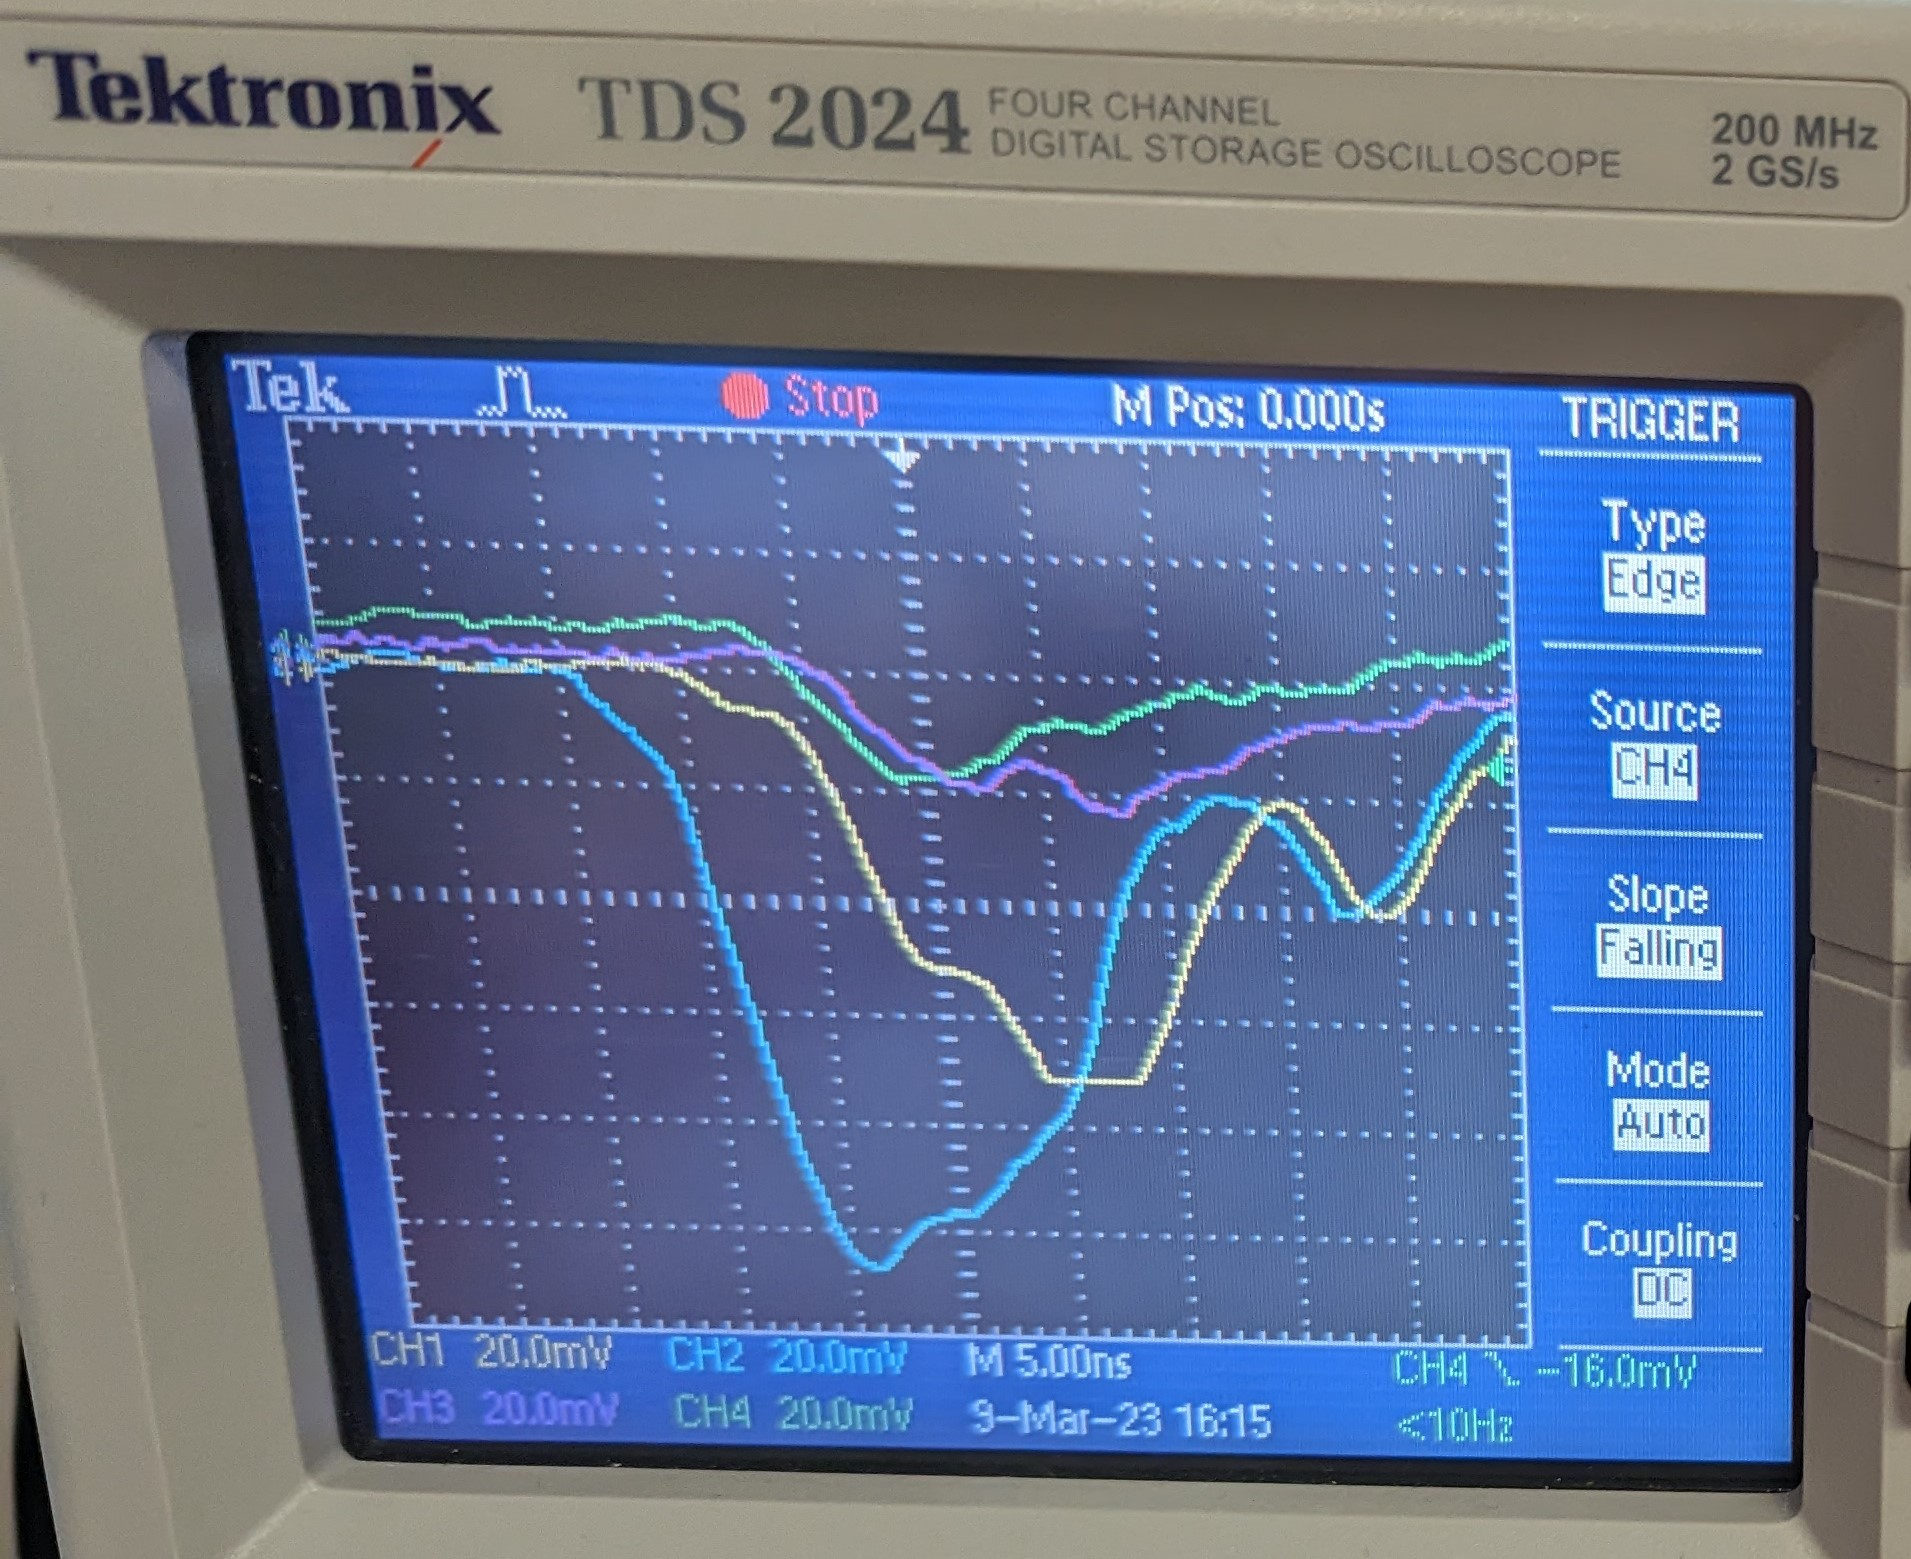
\includegraphics[width=0.55\linewidth]{images/afterpulseanalog.jpg}
    \caption{Oscilloscope observation of analogue signals from PMTs taken during first switching on of the system before calibration. In the cyan and yellow curves for example the peaks following the main one may have led to afterpulses, especially if the rising edge above threshold appears at the end of the LED signal.}
    \label{fig:analogafterpulse}
\end{figure}

\begin{figure}[htb!]
    \centering
    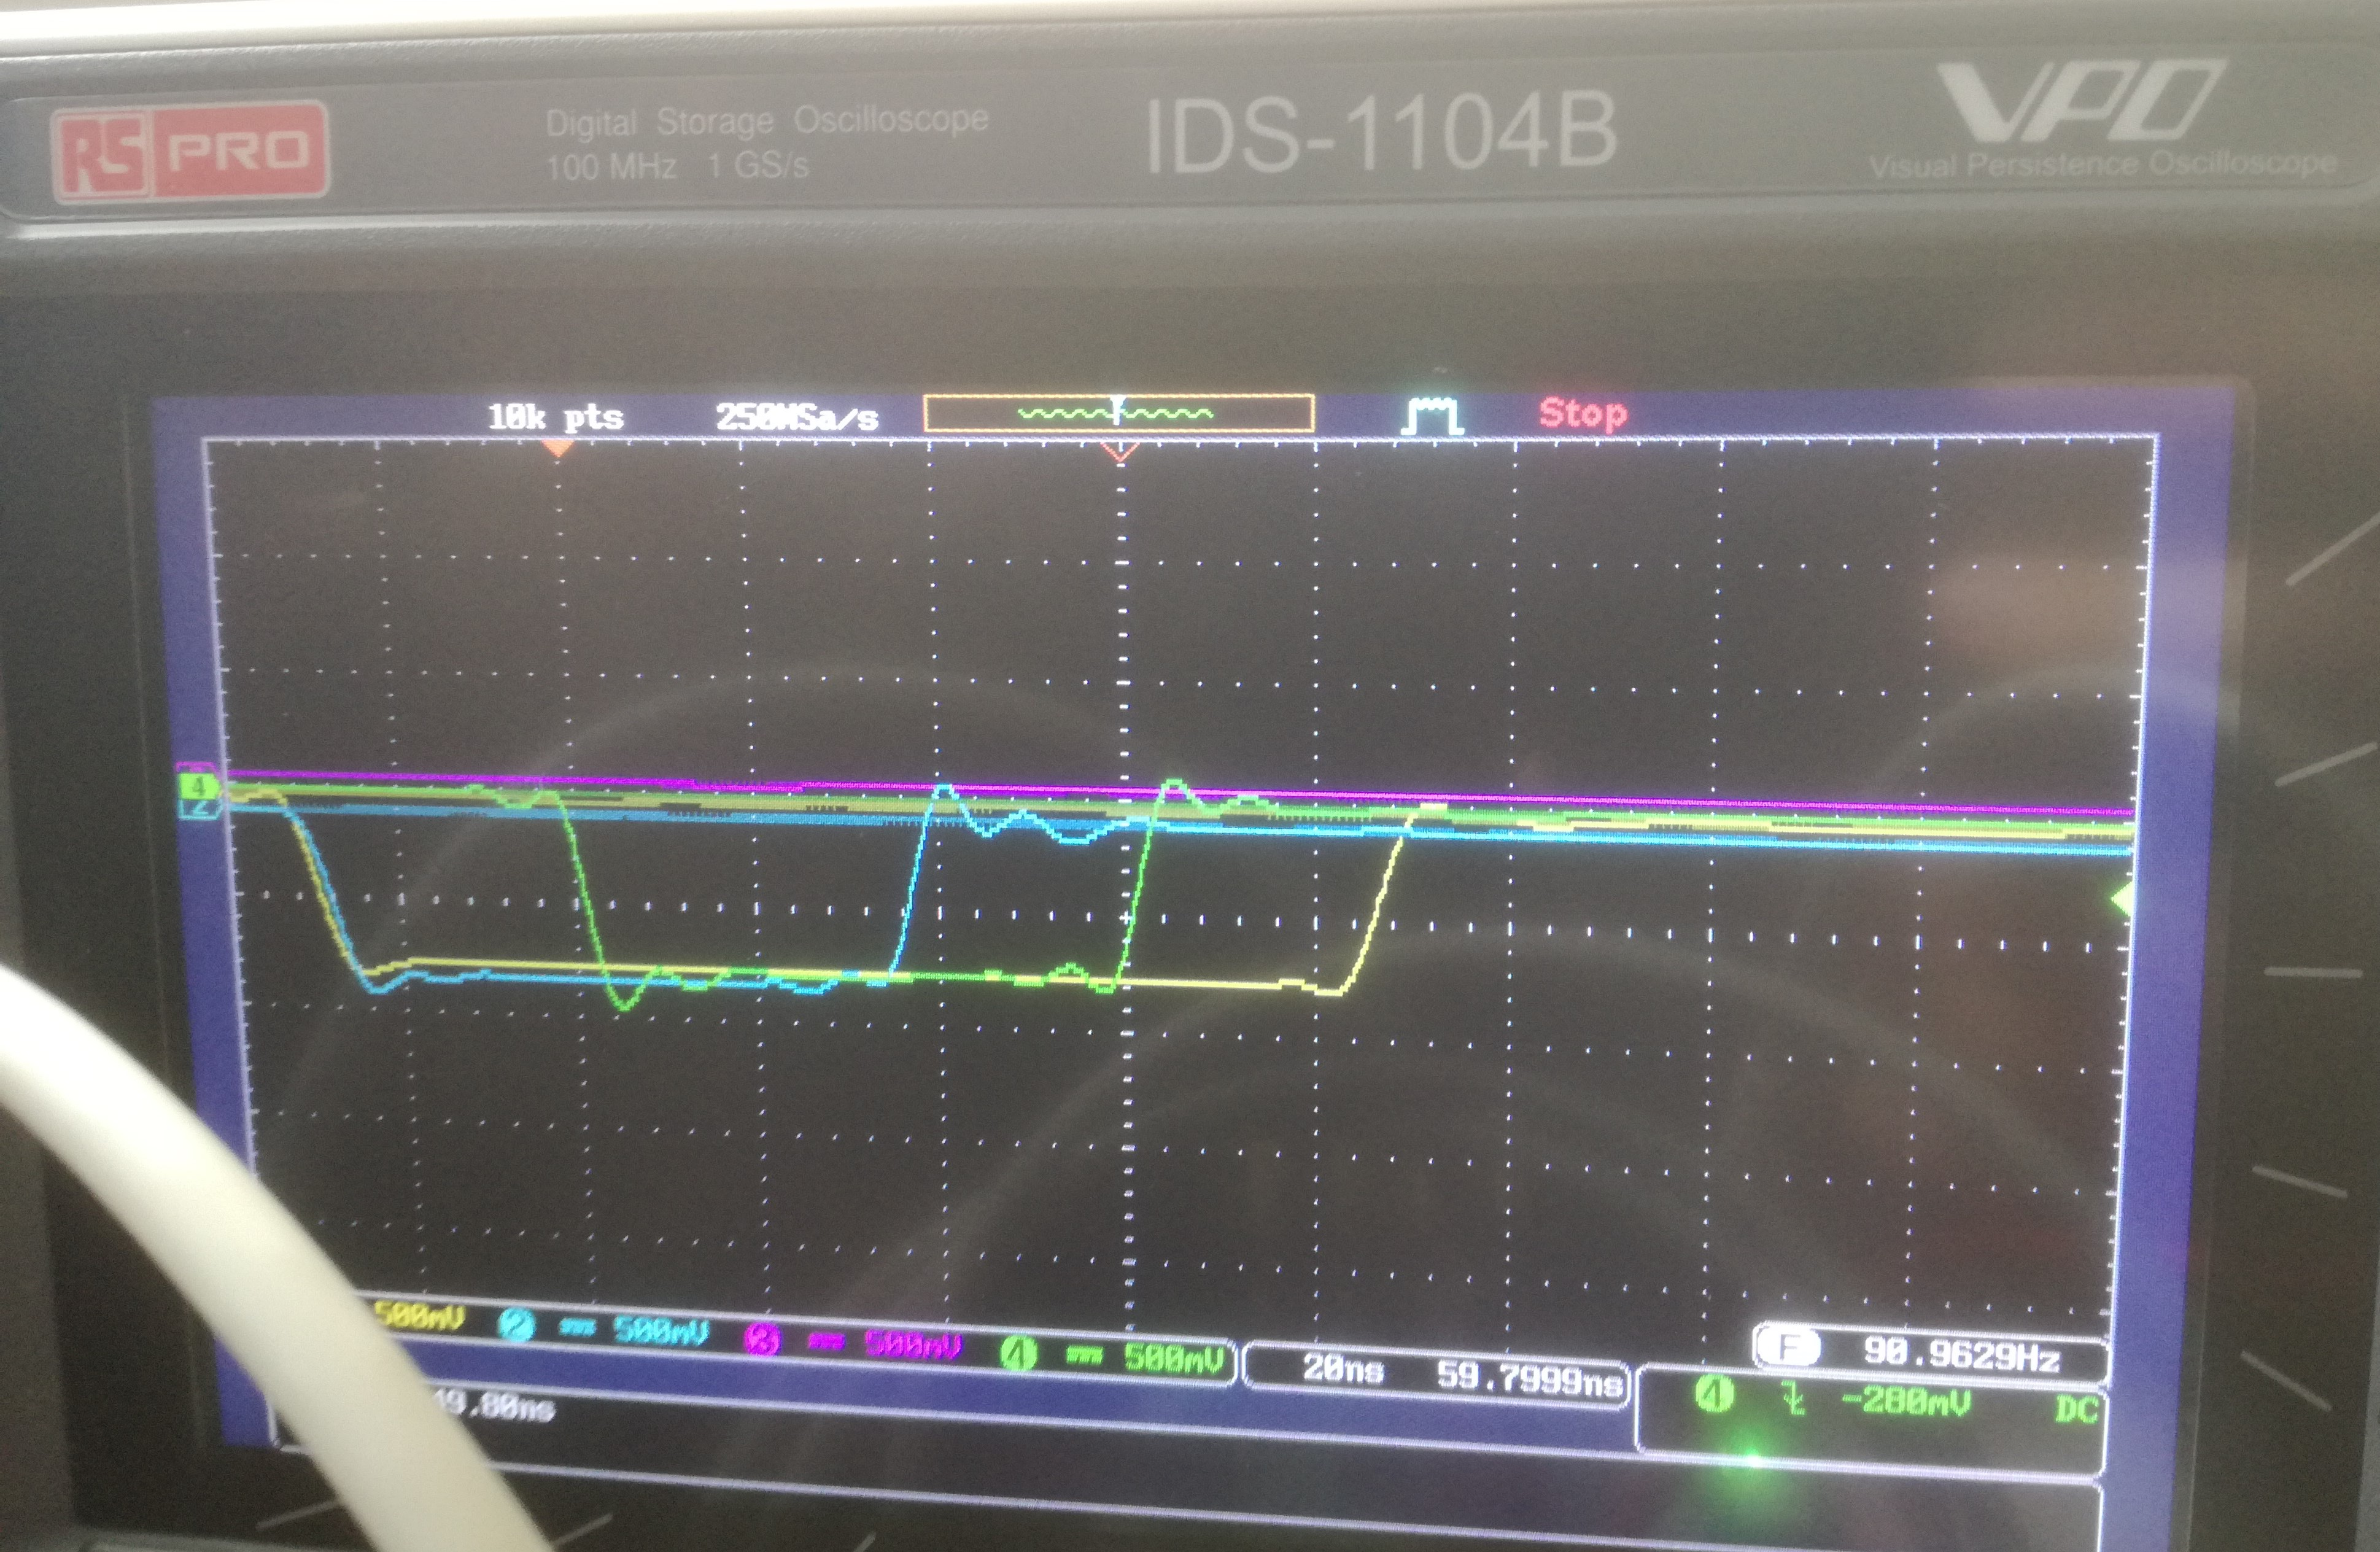
\includegraphics[width=0.65\linewidth]{images/afterpulse.jpg}
    \caption{Unexpected signal behaviour. The signal on CH1 (yellow) is set to last approximately as the one on CH2 (cyan). Instead it lasts longer then the trigger (green), and could cause an immediate stop on the event if it were not for the filters on the FPGA which should prevent the recording of this event. Other events showed a second rising front immediately after the lowering of the first signal. A signal of this second kind may survive the FPGA filter and get recorded as a valid stop.}
    \label{fig:afterpulse}
\end{figure}

Another possible reason for this behaviour may again be found in the too demanding settings of the PMTs. For instance, with the chosen working point, one of the PMTs of a plane may always be giving a signal, leading to fluctuations in the other PMT to survive the first AND in the logic circuit and giving out a signal. Furthermore, some other causes of error may be found in possible noise of the electronics.

\subsection{Events Selection}

Taking into account the previously discussed considerations, a proper event selection was done in order to perform the analysis. Since the acquisition program provides up to 3 stopping times, one for each scintillator plane, every time the trigger is activated and the expected decays happen in the absorber between P2 and P3, it would be reasonable to exclude from the analysis all events with a stopping time on P3 and at least one of the other 2 planes. In order to get rid of contaminated data also events with only stops on P1 or P2 were neglected during the analysis. Despite losing important statistics, with this approach it is possible to obtain extremely selected data. 

No further selection was applied on P3 since clear afterpulse-like effects were not visible. Reasons for the different behaviour of P3 may be either due to its PMTs working closer to their respective working point or, more likely, to the logic implemented in the trigger system. In fact, P3 acting as a veto implies it not being recently activated by the passage of the triggering muon and therefore being only sensitive to the effective passage of the ionising electron from the muon decay when afterpulsation effects are not happening.

\begin{figure}[htb!]
    \centering
    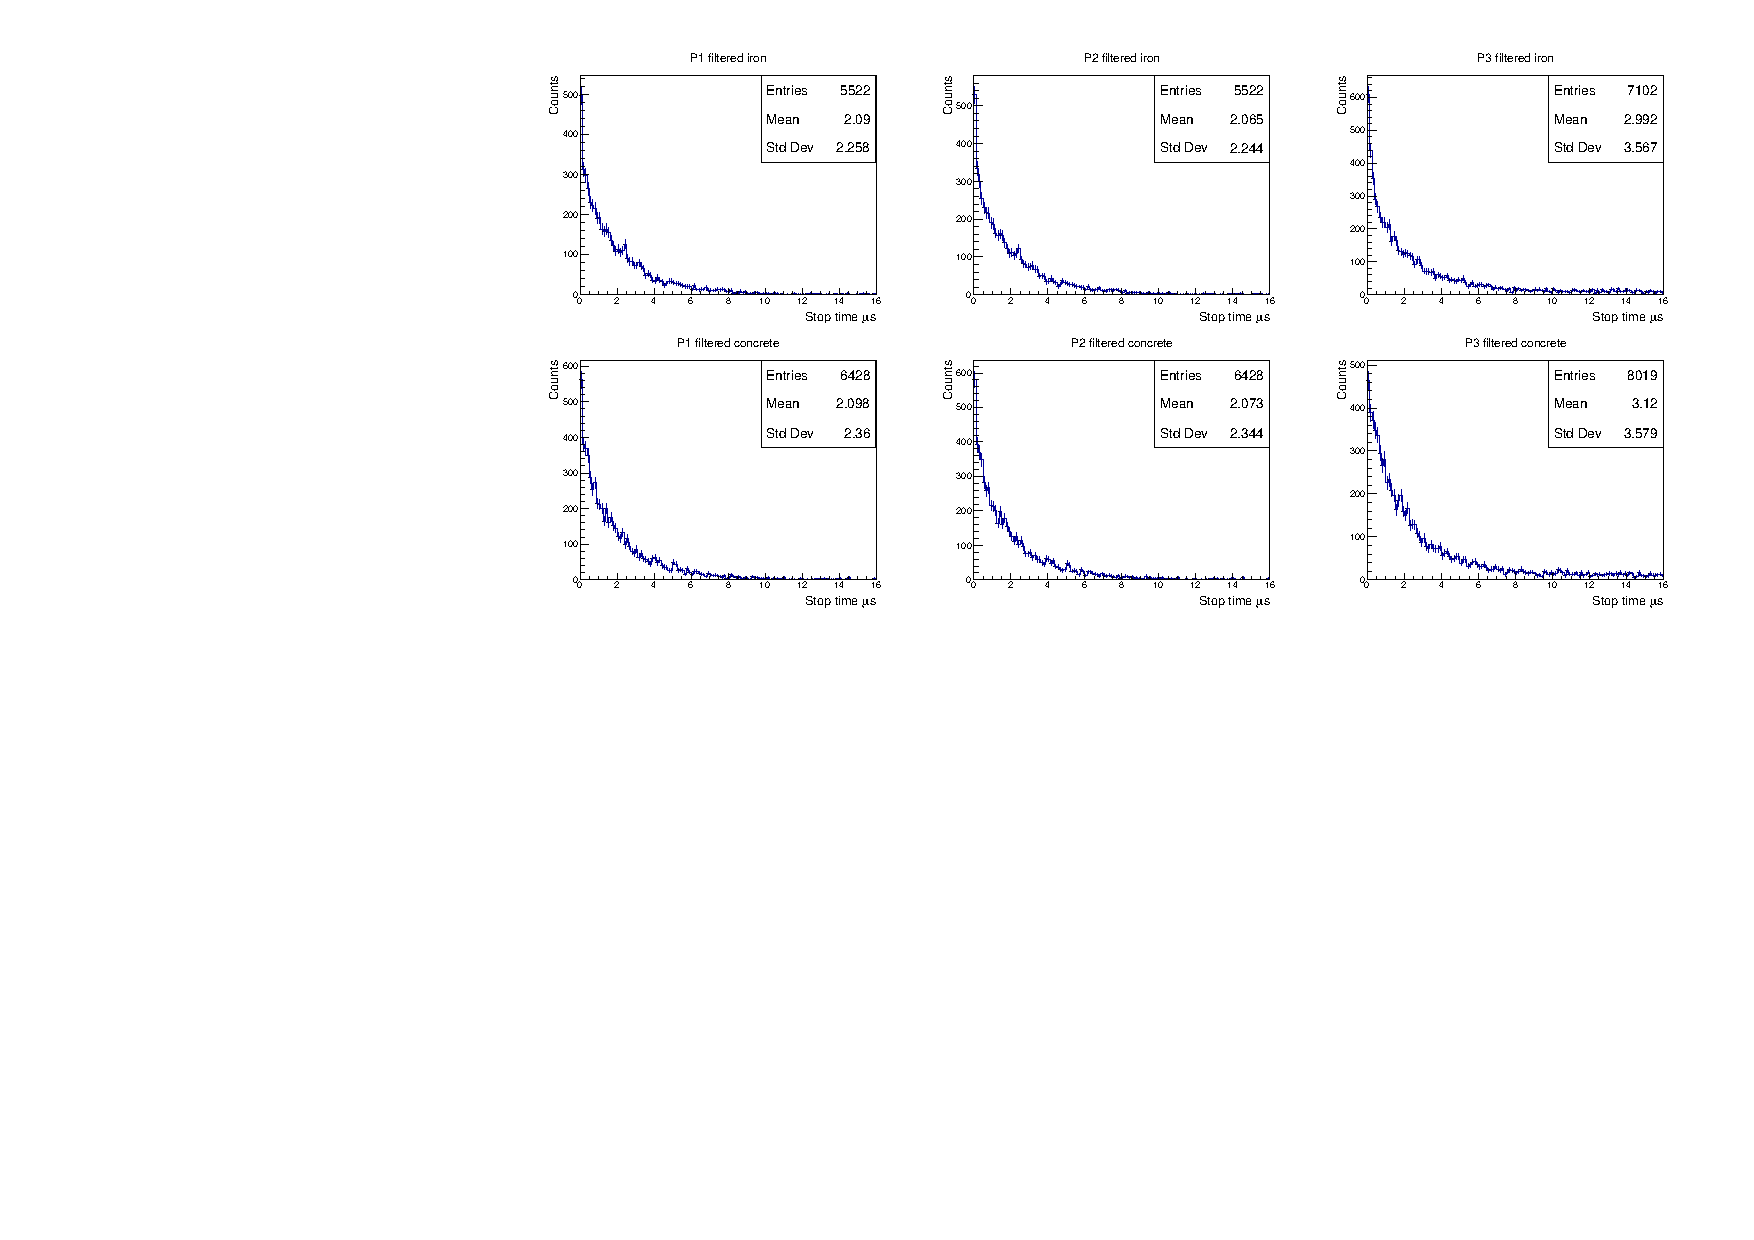
\includegraphics[width=\linewidth]{images/filtered_histograms.pdf}
    \caption{Histograms after applying the event selection. For P1 and P2 only events on both planes were considered.}
    \label{fig:filteredhistograms}
\end{figure}

The filtered histograms are available in Figure \ref{fig:filteredhistograms} and are the only ones actually used to perform the analysis. These histograms, compared to the raw ones of Figure \ref{fig:rawHisto}, do not show the unexpected peaks in the first bins. A closer look on the effects of events selection can be seen in Figures \ref{fig:150iron} and \ref{fig:150concrete}, where the first 150 bins are enlarged, having a width of 4 ns each, to observe how the unexpected peaks were removed and how P3 without filtering already resembled the behaviour of P1$\land$P2.

\subsection{Fitting}
\label{subsec:fitting}

Having performed event selection, it is possible to execute the final analysis. Firstly, a simple exponential fit with a free constant background term has been carried out. This choice for the background is motivated by the lack of sufficient statistics anticipated in Subsection \ref{subsec:bkg} and by the fact that we expect background sources from random coincidences once the trigger window has opened, leading to some sort of an exponential shape. At this point the flat behaviour may be easily justified by the expected timescale for such a background. Since the expected muon rate is around 1\,muon/\si{\centi \square \metre }/minute, we imagine the timescale for this process will be 3-4 orders of magnitude bigger than the \si{\micro \second} timescale of the muon decay we are trying to measure. Furthermore, random paired scintillation between the four PMTs of the coincidence planes should theoretically be rather infrequent. Finally, for the first fit, we are left with equation (\ref{eq:simpleExp}).
\begin{equation}
    f(t)=N_0 \exp{-\frac{t}{\tau_0}}+b
    \label{eq:simpleExp}
\end{equation}

\begin{figure}[htb!]
    \centering
    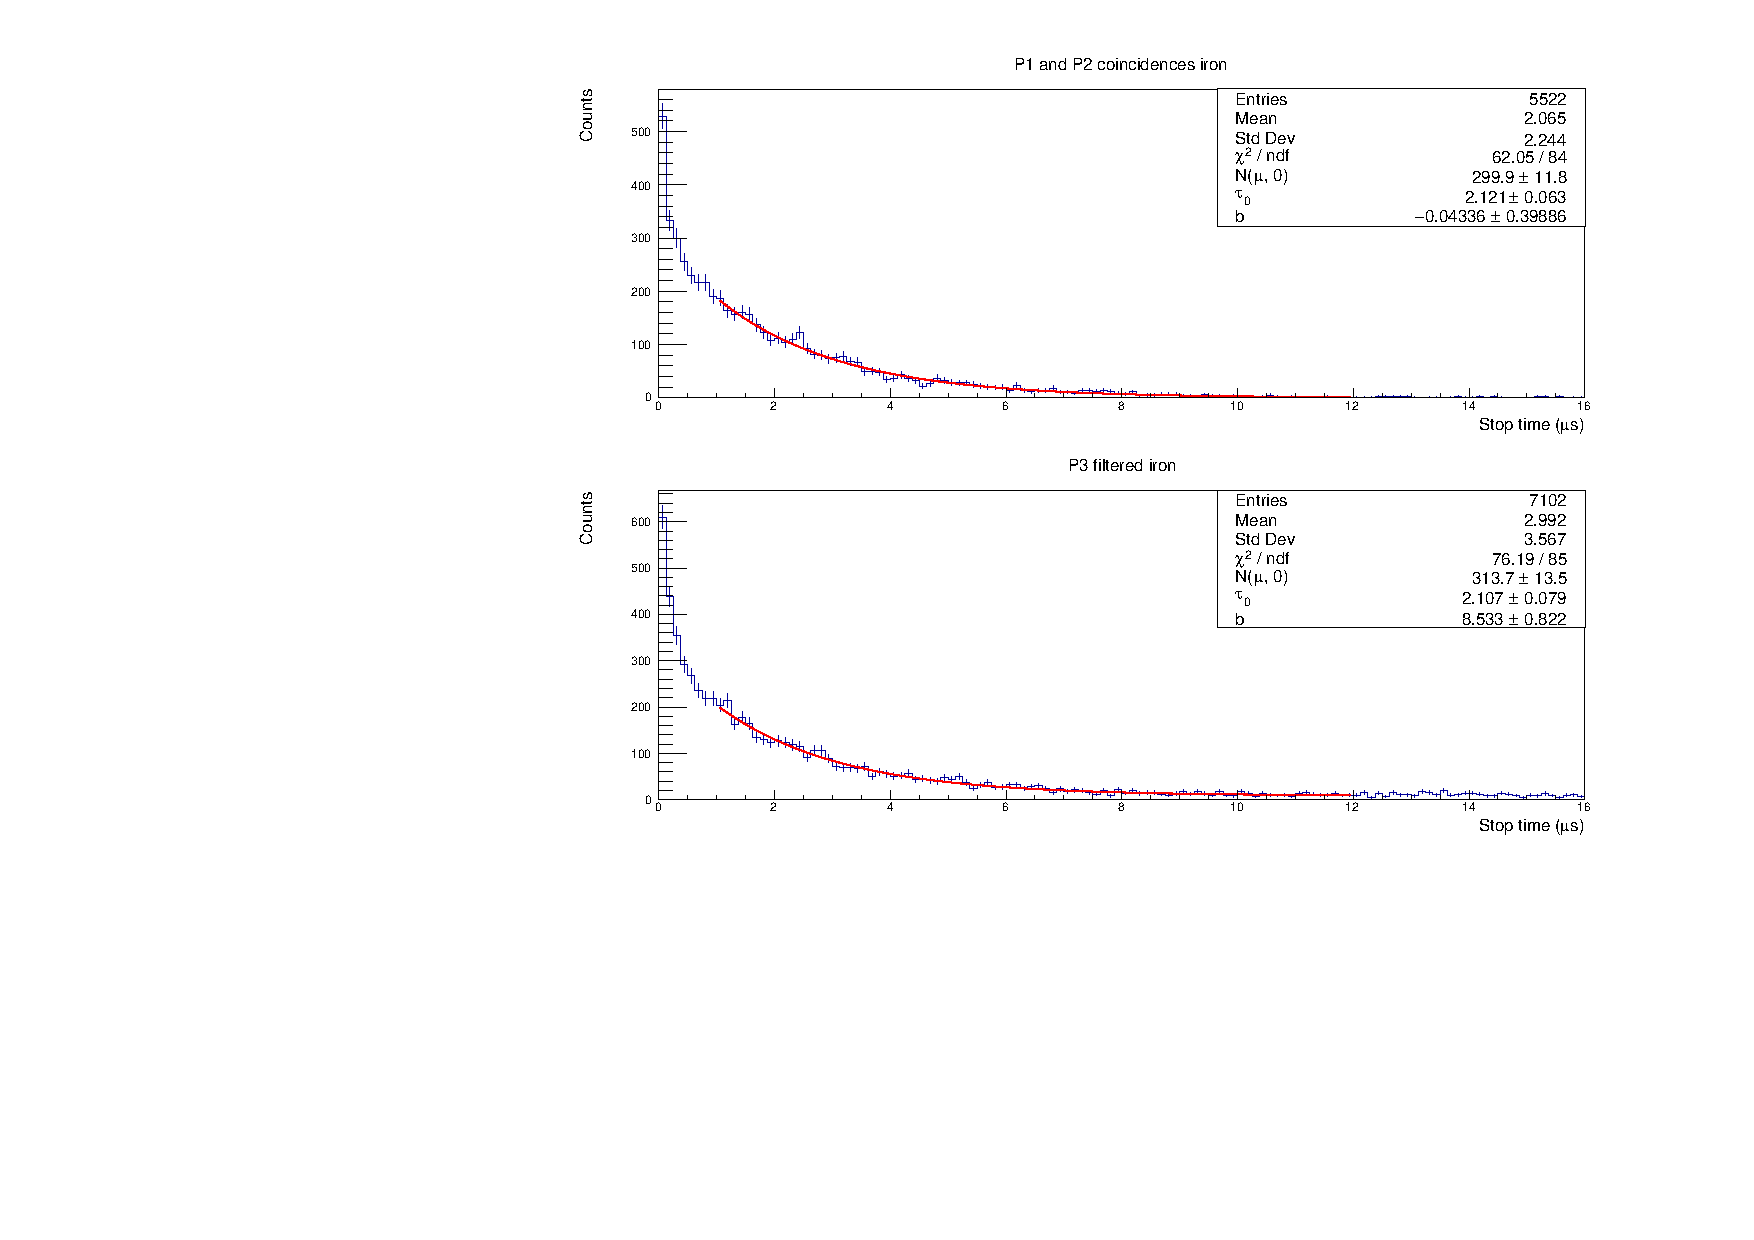
\includegraphics[width=0.9\linewidth]{images/iron_filtered_fit.pdf}
    \caption{Simple exponential fits for the iron absorber. The fit range has been adjusted to reduce the impact of muon capture by nuclei.}
    \label{fig:ironFits}
\end{figure}

\begin{figure}[htb!]
    \centering
    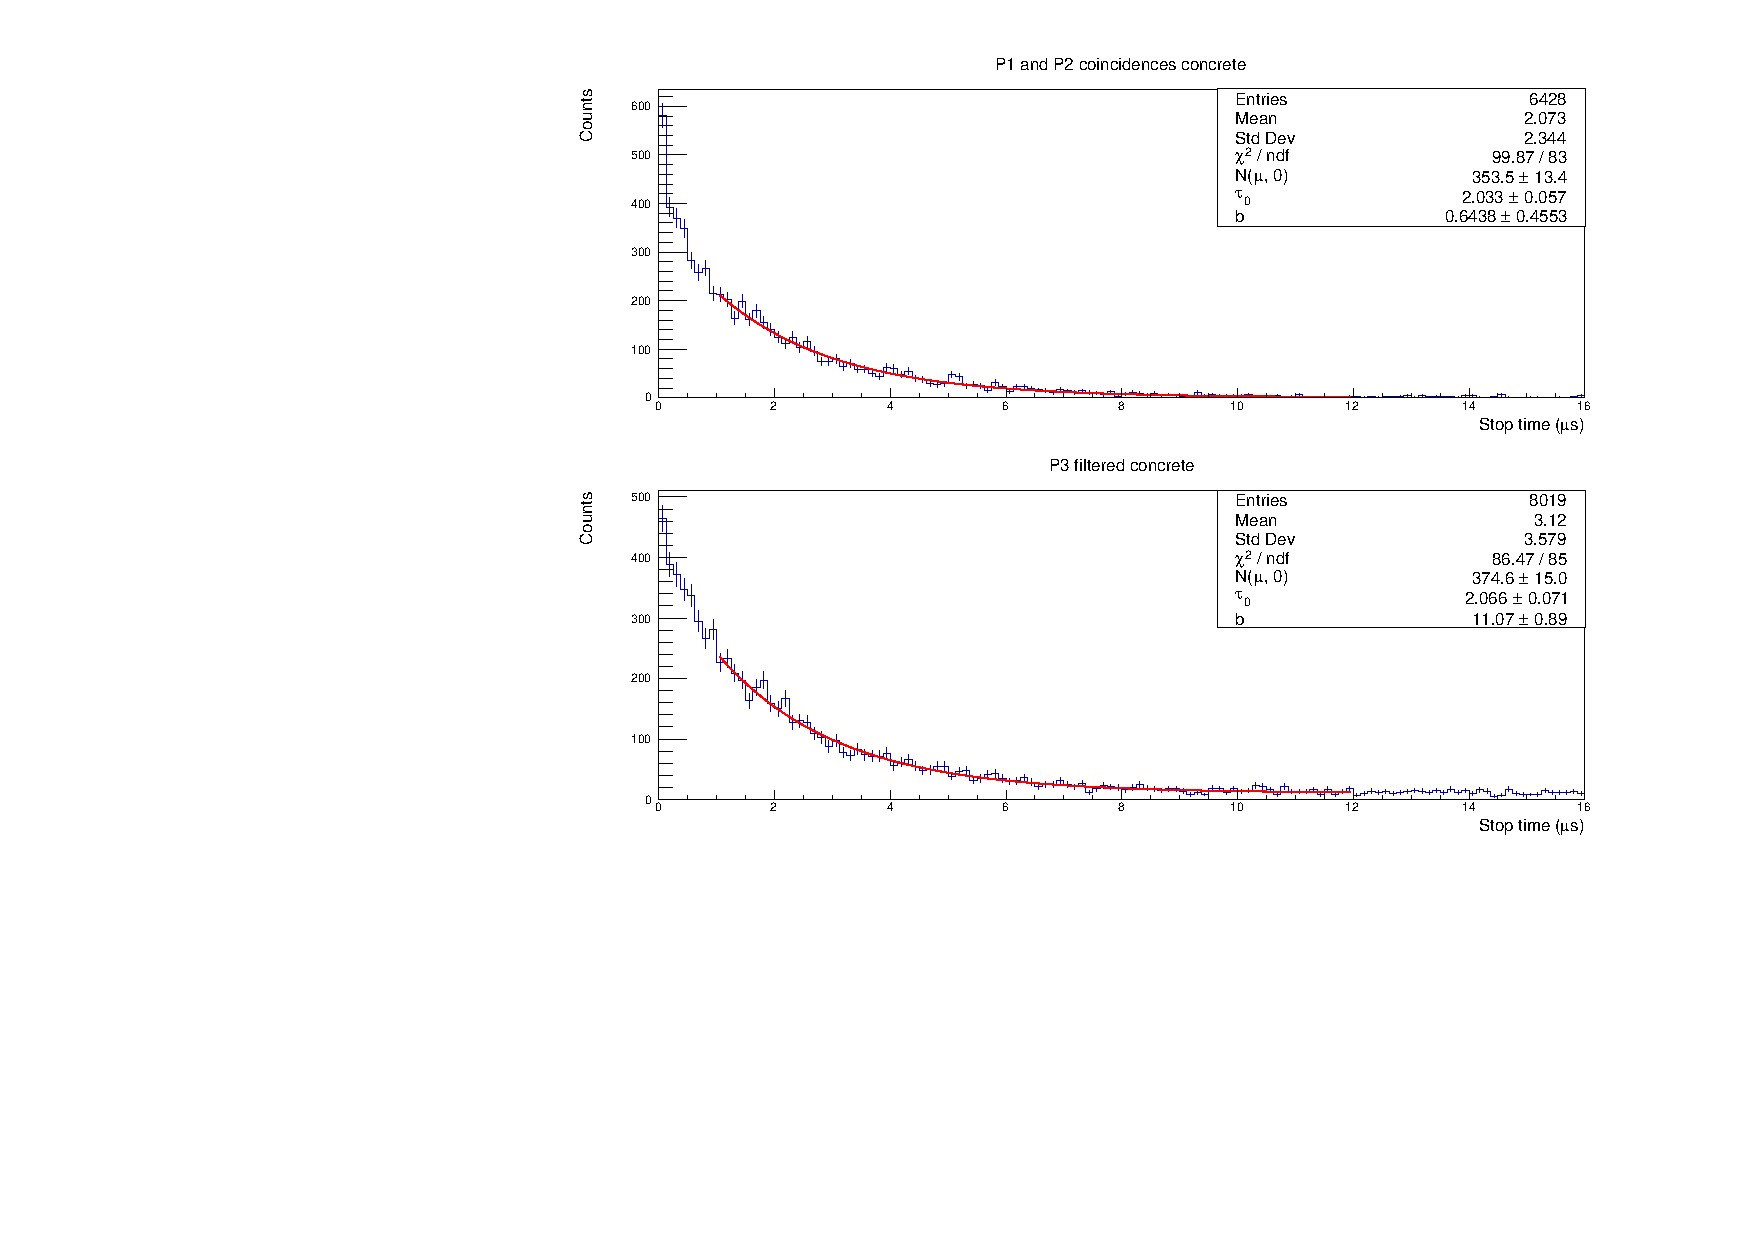
\includegraphics[width=0.9\linewidth]{images/concrete_filtered_fit.pdf}
    \caption{Simple exponential fits for the concrete absorber. The fit range has been adjusted to reduce the impact of muon capture by nuclei. Note that the choice to use a different starting point with respect to iron is due to a significant difference in mean capture time ($\approx$200\,ns in iron versus $\approx$1\,$\mu$s in concrete).}
    \label{fig:concreteFits}
\end{figure}

The results of the fits can be seen in Figures \ref{fig:ironFits} and \ref{fig:concreteFits}. The first thing that can be noticed is how well the event selection on P1 and P2 gets rid of the background, which is almost an order of magnitude smaller compared to the unfiltered events in P3. Moreover the quality of fit is rather good, having a $\Tilde{\chi^2}$ value around 1. In fact, according to the Pearson's $\chi^2$ statistics \cite{pearson1900x}, the $\chi^2$ \footnote{$=\sum_i (n_i - \nu_i)^2/\sigma_i^2$ In the case under study dealing with poissonian counting $\sigma_i^2=\nu_i.$} should follow a distribution whose expectation value is the number of degrees of freedom, hence a $\Tilde{\chi^2}$ close to unity suggests a good quality of fit. Estimated muon lifetimes from the  simple exponential fits are shown in Table \ref{tab:resultsSimple}, combined results are obtained via least squares combination techniques\footnote{$\hat{\lambda}=\sum_i(y_i/\sigma_i^2)/\sum_i(1/\sigma_i^2)$;\hspace{0.1cm} $\sigma^2_{\lambda}=1/\sum_i(1/\sigma_i^2)$}.

\begin{table}[htb!]
    \caption{Results of the simple exponential fit of the filtered data for first measurement of the muon lifetime. Combined results refers to cumulative data combined via the least squares technique.}
    \label{tab:resultsSimple}
    \centering
        \begin{tabular}{|l|c|}
        \hline
        Plane & $\tau_0$ estimate [\si{\micro \second}] \\ \hline
        P1 $\land$ P2 iron        & 2.055 $\pm$ 0.042 \\
        P3 iron           & 2.061 $\pm$ 0.051 \\
        P1 $\land$ P2 concrete    & 1.994 $\pm$ 0.046 \\
        P3 concrete       & 2.083 $\pm$ 0.060 \\ \hline
        Iron cumulative     & 2.087 $\pm$ 0.034 \\
        Concrete cumulative & 2.064 $\pm$ 0.039 \\ \hline
        Combined & 2.070 $\pm$ 0.030 \\ \hline
        \end{tabular}
\end{table}

\FloatBarrier

Another thing worth noting is that estimated muon lifetime $\tau_0$ from single fits is not compatible with the known value within one standard deviation suggesting the action of some sort of effects, as all the estimated parameters are lower than the currently known value. This is especially evident from the combined fit result for $\tau_0$. For what concerns this lowering of the muon lifetime the effect can be partially due to the different behaviour of oppositely charged muons, as $\mu^-$ can undergo atomic capture. Because of this effect, their lifetime should be reduced to a $\tau_{eff}$ according to (\ref{eq:taueff}), where $\tau_c$ is the characteristic absorption time scale of the absorber.

\begin{equation}
    \frac{1}{\tau_{eff}} = \frac{1}{\tau_0}+\frac{1}{\tau_c}
    \label{eq:taueff}
\end{equation}

In order to account for different behaviours of differently charged muons, the final fit expression should be modified. Using $R$ atmospheric muon charge ratio as shown in (\ref{eq:r}) the final fit expression should become (\ref{eq:finalFit}).

\begin{equation}
\label{eq:r}
    R = \frac{N(\mu^+)}{N(\mu^-)} = \frac{\textnormal{\# positive }\mu}{\textnormal{\# negative }\mu}
\end{equation}

\begin{equation}
\label{eq:finalFit}
    N(t) = N_0 \exp{-\frac{t}{\tau_0}}(1+\frac{1}{R}\exp{-\frac{t}{\tau_c}})+b
\end{equation}

A first approach to using this formula for the fit led to Figures \ref{fig:allFreeIron} and \ref{fig:allFreeConcrete}, for which all the parameters have been left free. In order to try to improve the results, the muon lifetime has been fixed to the currently known value to get better estimates of $R$ and $\tau_c$. Ideally, this procedure may have been simplified by a proper background measurement which would have allowed to remove the background $b$ parameter. The results are shown in Figures \ref{fig:fixedIron} and \ref{fig:fixedConcrete}. The combined fit results can be found in Tables \ref{tab:t0RFit} and \ref{tab:tauCResults}. The constraint on $\tau_0$ has allowed to reach values of muon capture times compatible with the expected values $\tau_{C\textnormal{ iron}}$, $\tau_{C\textnormal{ concrete}}$ given by \cite{nayel2018characterisation,suzuki1987total}. However, the better estimate of the atmospheric muon charge ratio comes from the free fit and that value has been chosen as final result presented by this work as it is in agreement with the CMS measurement of $R$ \cite{khachatryan2010measurement}. Final results from simple exponential fit, free fit and constrained fit are:
\begin{alignat*}{3}
    &\tau_0 &=2.120\phantom{0}&\pm 0.037\, \si{\micro \second} \\
    &R & =1.26\phantom{00}&\pm 0.30\phantom{0} \\
    &\tau_{C\textnormal{ iron}} & =0.2478&\pm 0.0645\, \si{\micro \second} \\
    &\tau_{C\textnormal{ concrete}} & =1.133\phantom{0}&\pm 0.333\phantom{0}\, \si{\micro \second}.
\end{alignat*}

\FloatBarrier
\begin{figure}[htb!]
    \centering
    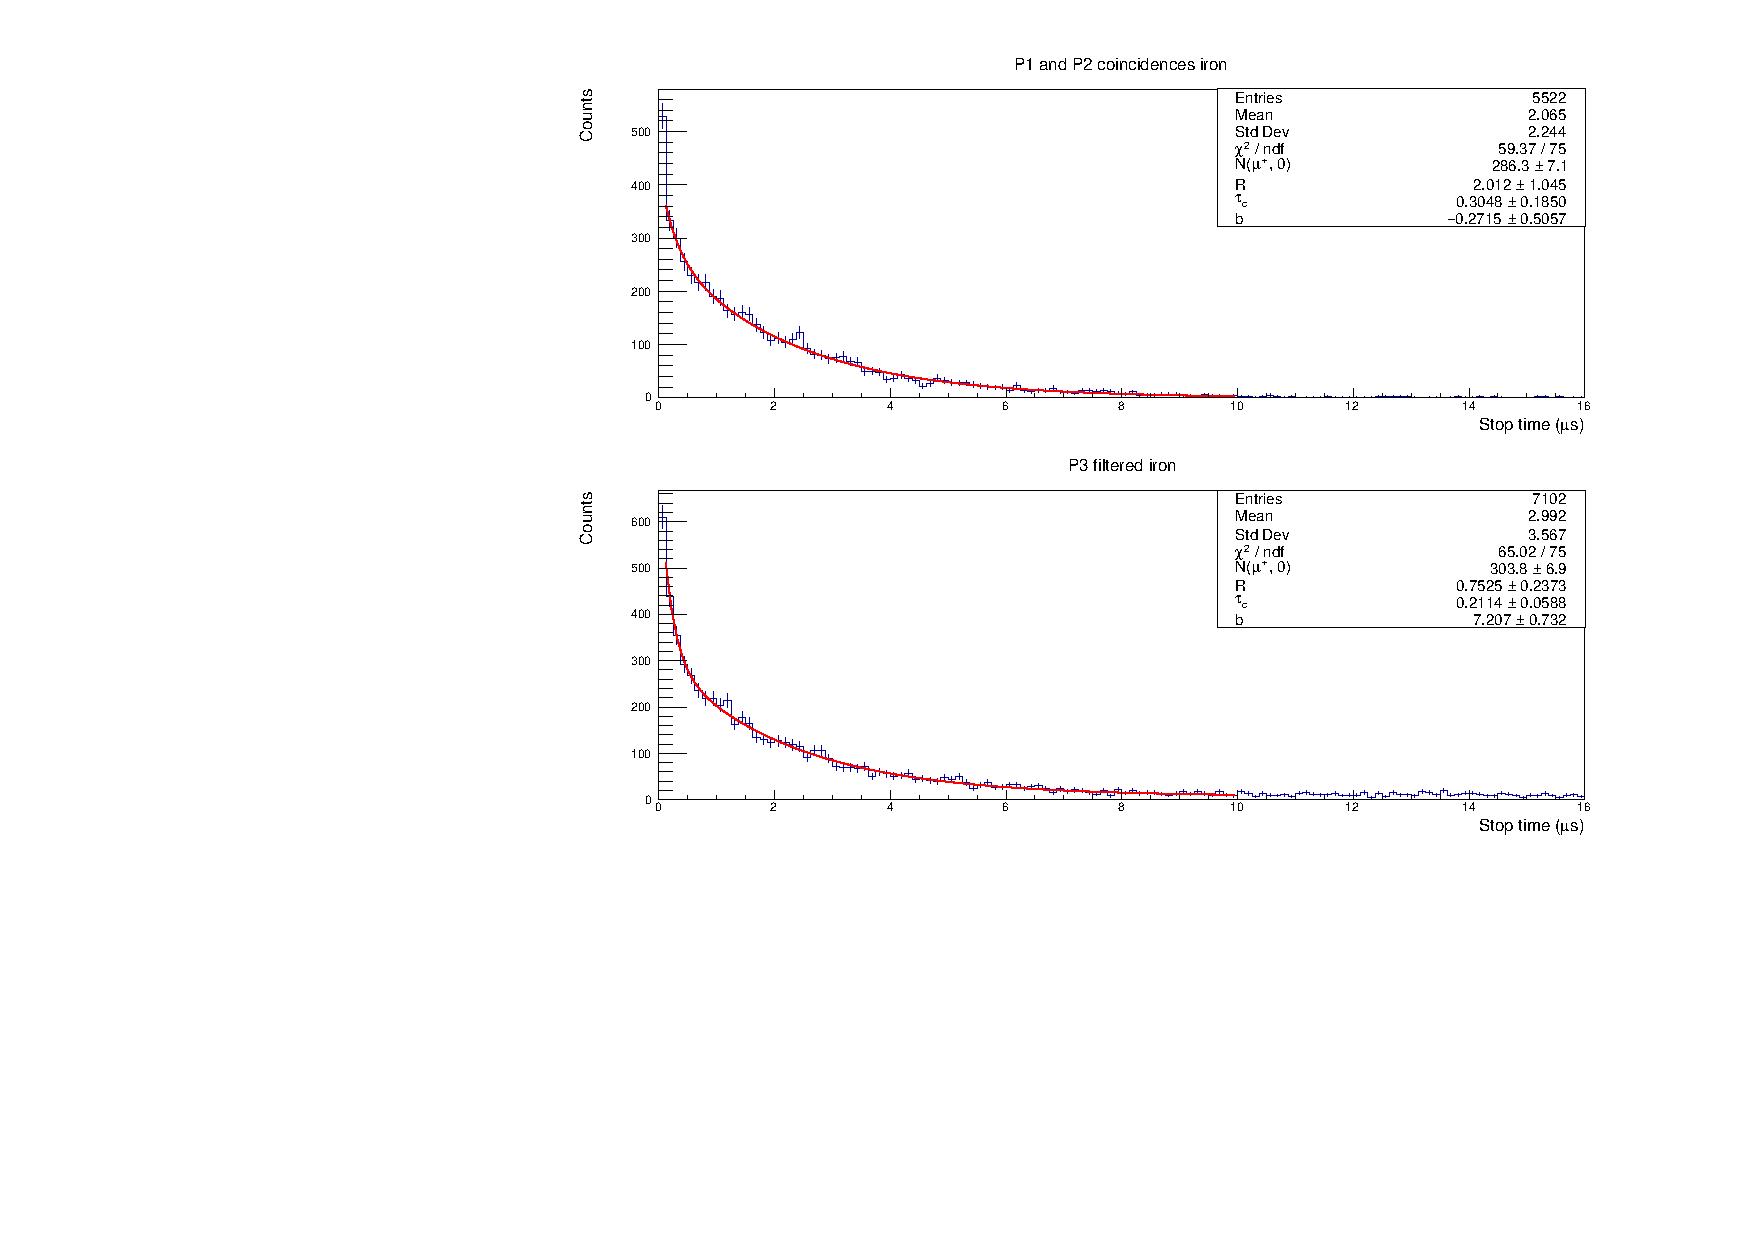
\includegraphics[width=0.9 \linewidth]{images/fixed_lifetime_fit_iron.pdf}
    \caption{Fit for the iron absorber accounting for different charge muon behaviours with fixed muon lifetime.}
    \label{fig:fixedIron}
\end{figure}

\begin{figure}[htb!]
    \centering
    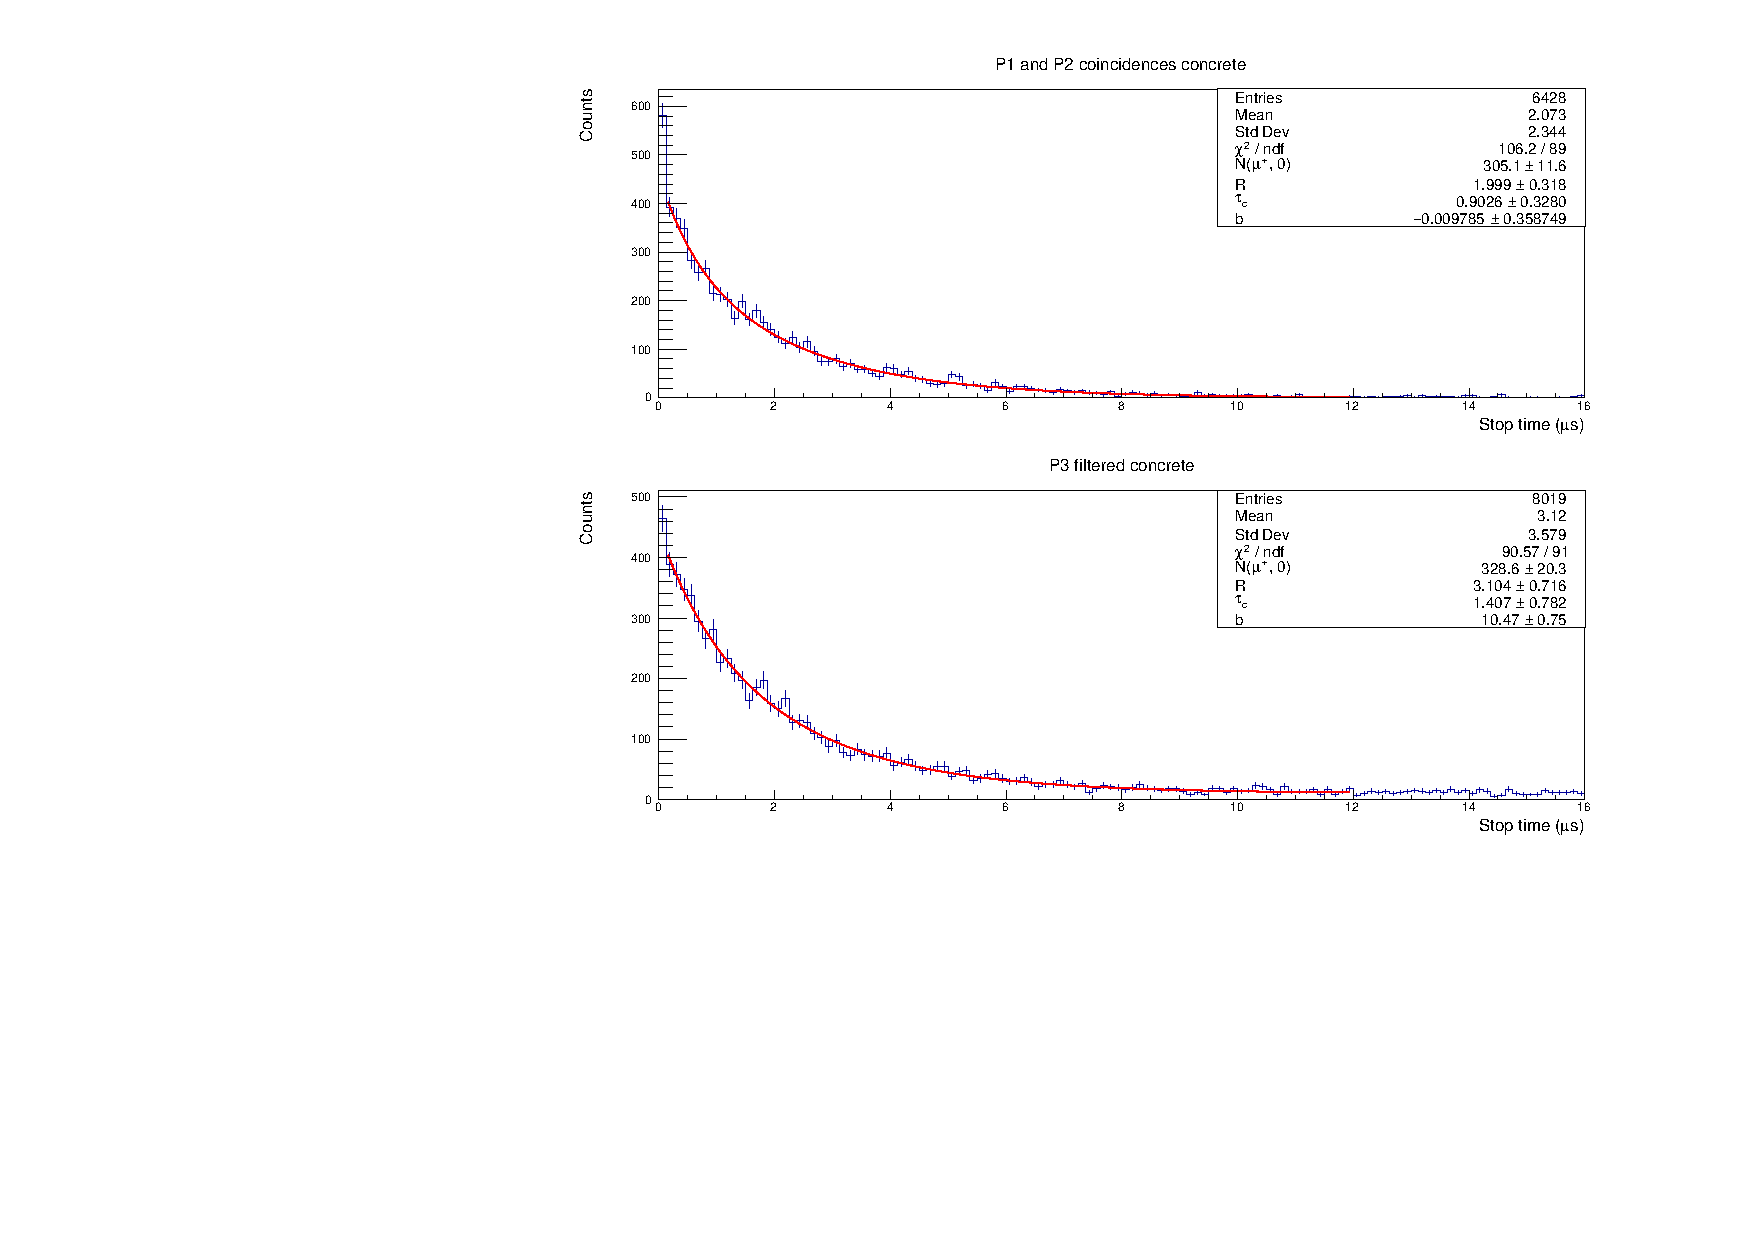
\includegraphics[width=0.9 \linewidth]{images/fixed_lifetime_fit_concrete.pdf}
    \caption{Fit for the concrete absorber accounting for different charge muon behaviours with fixed muon lifetime.}
    \label{fig:fixedConcrete}
\end{figure}
\FloatBarrier

\begin{table}[htb!]
        \caption{Results of the fits accounting for different muon charges. (All) refers to the fit with all parameters left free, (Constrained) refers to the fit in which $\tau_0$ is fixed to the currently known value (considered without error at our precision). Combined results refers to cumulative data combined via the least squares technique. Highlighted values are the final results presented in this work.}
    \label{tab:t0RFit}
        \centering
        \begin{tabular}{|l|cc|c|}
        \hline
        Plane             & $\tau_0$ (All) [\si{\micro \second}]         & $R$ (All)            & $R$ (Constrained) \\ \hline
        P1 $\land$ P2 iron     & 2.062 $\pm$ 0.046 & 1.569 $\pm$ 1.255     & 2.456 $\pm$ 1.551     \\
        P3 iron             & 2.108 $\pm$ 0.062 & 0.712 $\pm$ 0.255 & 0.786 $\pm$ 0.236   \\ 
        Iron cumulative & 2.118 $\pm$ 0.041 & 0.991 $\pm$ 0.322 & 1.12\phantom{0} $\pm$ 0.30\phantom{0} \\ \hline
        P1 $\land$ P2 concrete & 2.012 $\pm$ 0.058 & 2.514 $\pm$ 0.821   & 1.883 $\pm$ 0.260     \\
        P3 concrete         & 2.156 $\pm$ 0.150 & 3.7\phantom{00} $\pm$ 2.6\phantom{00}     & 3.1\phantom{00} $\pm$ 0.7\phantom{00}     \\ 
        Concrete cumulative & 2.127 $\pm$ 0.081 & 3.049 $\pm$ 0.830 & 2.49\phantom{0} $\pm$ 0.30\phantom{0} \\ \hline
        Combined            & \cellcolor[HTML]{67FD9A}2.120 $\pm$ 0.037 & \cellcolor[HTML]{67FD9A}1.26\phantom{0}  $\pm$ 0.30\phantom{0}   & 1.81\phantom{0}  $\pm$ 0.21\phantom{0}      \\
        Expected \cite{khachatryan2010measurement, Workman2022ynf}           & 2.197 \phantom{$\pm$ 0.000}        & 1.277 $\pm$ 0.005   & 1.277 $\pm$ 0.005     \\ \hline
        \end{tabular}
\end{table}

\begin{table}[htb!]
        \centering
    \caption{Capture rate of negative muons estimated from the fits accounting for different muon charges for the two different absorbers (iron and concrete). (All) refers to the fit with all parameters left free, (Constr) refers to the fit in which $\tau_0$ is fixed to the currently known value (considered without error at our precision). Expected values are taken from \cite{suzuki1987total} for pure iron and roughly estimated using \cite{nayel2018characterisation, suzuki1987total} for concrete. Knowing the precise concrete composition would drastically improve this estimate. Highlighted values are the final results presented in this work.}
    \label{tab:tauCResults}
    \resizebox{\textwidth}{!}{
        \begin{tabular}{|l|cc|cc|}
        \hline
        Plane & $\tau_{C\textnormal{iron}}$ (All) [\si{\micro \second}] & $\tau_{C\textnormal{iron}}$ (Constr) [\si{\micro \second}] & $\tau_{C\textnormal{concr}}$ (All) [\si{\micro \second}] & $\tau_{C\textnormal{concr}}$ (Constr) [\si{\micro \second}] \\ \hline
        P1 $\land$ P2 & 0.1625 $\pm$ 0.0985  & 0.4652 $\pm$ 0.5003 & 0.4102 $\pm$ 0.2046 & 1.281 $\pm$ 0.516  \\
        P3 & 0.1852 $\pm$ 0.0583 & 0.2314 $\pm$ 0.0646 & 1.179\phantom{0} $\pm$ 1.044\phantom{0} & 1.413 $\pm$ 0.735 \\\hline
        Cumulative & 0.1879 $\pm$ 0.0538   & \cellcolor[HTML]{67FD9A}0.2478 $\pm$ 0.0645 & 0.8205 $\pm$ 0.4330 & \cellcolor[HTML]{67FD9A}1.133 $\pm$ 0.333  \\
        Expected   & 0.206 $\pm$ 0.001 & 0.206\phantom{0} $\pm$ 0.001\phantom{0} & 1.2\phantom{000} $\pm$ 0.3\phantom{000}             & 1.2\phantom{00} $\pm$ 0.3\phantom{00}                  \\ \hline
        \end{tabular}
        }
\end{table}

\end{document}
\clearpage